\documentclass{article}

\usepackage{textcomp}
\usepackage{fontenc}

\usepackage{graphicx}
\usepackage{caption}
\usepackage{gensymb} % for \degree
\usepackage{placeins} % for \images
\usepackage[margin=1in]{geometry} % to set margins

\bibliographystyle{naturemag}

\renewcommand{\familydefault}{\sfdefault}
\graphicspath{{images/}}	% Root directory of the figures
\setlength{\parskip}{2 mm}

%\bibliography{/Users/danflynn/Dropbox/References/Bibrefs/danlib}
%\bibliographystyle{naturemag}


\usepackage{Sweave}
\begin{document}

\Sconcordance{concordance:SuppMat_Budburst.tex:SuppMat_Budburst.Rnw:%
1 16 1 1 0 29 1 1 13 1 45 38 0 1 2 1 24 24 0 1 2 1 7 24 0 1 3 84 1}
 % set to F?


\flushleft

\textbf{\large{Supplemental Materials: Photoperiod and temperature interactively drive spring phenology in multiple species}}

Flynn, Wolkovich...

\textit{The Arnold Arboretum of Harvard University}

%% Add S prefix for tables and figures in Supplemental Materials
\renewcommand{\thetable}{S\arabic{table}}
\renewcommand{\thefigure}{S\arabic{figure}}

%%%%%%%%%%%%%%%%%%%%%%%%%%%%%%%
\section*{Supplemental Figures and Tables}
%%%%%%%%%%%%%%%%%%%%%%%%%%%%%%%


% latex table generated in R 3.2.3 by xtable 1.7-4 package
% Mon Apr 25 15:36:27 2016
\begin{table}[ht]
\centering
\caption{Summary of mixed effect model of budburst day by species.} 
\begin{tabular}{rrrrrrr}
  \hline
 & mean & sd & 25\% & 50\% & 75\% & Rhat \\ 
  \hline
Temperature & -6.80 & 1.71 & -7.95 & -7.02 & -5.63 & 1.05 \\ 
  Photoperiod & -3.96 & 1.67 & -5.13 & -4.13 & -2.80 & 1.05 \\ 
  Chilling 4 \degree C & -22.09 & 2.84 & -24.05 & -21.75 & -20.26 & 1.03 \\ 
  Chilling 1.5 \degree C & -19.79 & 2.96 & -22.32 & -19.90 & -17.78 & 1.13 \\ 
  Site & 2.59 & 1.88 & 0.93 & 2.54 & 3.93 & 1.13 \\ 
  Temperature $\times$ Photoperiod & -0.60 & 0.72 & -1.07 & -0.46 & -0.24 & 1.02 \\ 
  Temperature $\times$ Site & -1.48 & 0.76 & -1.99 & -1.35 & -1.00 & 1.04 \\ 
  Photoperiod $\times$ Site & 0.05 & 0.79 & -0.52 & 0.09 & 0.76 & 1.10 \\ 
  Temperature $\times$ Chilling 4 \degree C & 9.17 & 1.00 & 8.50 & 9.32 & 9.77 & 1.03 \\ 
  Temperature $\times$ Chilling 1.5 \degree C & 9.68 & 1.06 & 9.11 & 9.57 & 10.33 & 1.00 \\ 
  Photoperiod $\times$ Chilling 4 \degree C & -0.18 & 0.96 & -0.82 & -0.06 & 0.47 & 1.04 \\ 
  Photoperiod $\times$ Chilling 1.5 \degree C & -0.02 & 1.03 & -0.67 & 0.14 & 0.48 & 1.02 \\ 
  Site $\times$ Chilling 4 \degree C & -1.96 & 1.33 & -2.84 & -1.86 & -0.85 & 1.09 \\ 
  Site $\times$ Chilling 1.5 \degree C & -3.49 & 1.23 & -4.14 & -3.55 & -2.78 & 1.01 \\ 
   \hline
\end{tabular}
\end{table}
% latex table generated in R 3.2.3 by xtable 1.7-4 package
% Mon Apr 25 15:36:27 2016
\begin{table}[ht]
\centering
\caption{Summary of mixed effect model of leafout day by species.} 
\begin{tabular}{rrrrrrr}
  \hline
 & mean & sd & 25\% & 50\% & 75\% & Rhat \\ 
  \hline
Temperature & -21.91 & 1.72 & -23.05 & -21.90 & -20.75 & 1.01 \\ 
  Photoperiod & -13.68 & 1.69 & -14.79 & -13.71 & -12.56 & 1.02 \\ 
  Chilling 4 \degree C & -26.37 & 3.09 & -28.41 & -26.41 & -24.41 & 1.01 \\ 
  Chilling 1.5 \degree C & -26.14 & 3.09 & -28.29 & -26.23 & -24.03 & 1.01 \\ 
  Site & 3.00 & 2.05 & 1.67 & 3.00 & 4.43 & 1.02 \\ 
  Temperature $\times$ Photoperiod & 3.54 & 0.77 & 2.99 & 3.54 & 4.07 & 1.02 \\ 
  Temperature $\times$ Site & -0.59 & 0.82 & -1.11 & -0.58 & -0.04 & 1.03 \\ 
  Photoperiod $\times$ Site & -1.00 & 0.83 & -1.55 & -1.01 & -0.42 & 1.02 \\ 
  Temperature $\times$ Chilling 4 \degree C & 10.19 & 1.16 & 9.47 & 10.12 & 10.93 & 1.00 \\ 
  Temperature $\times$ Chilling 1.5 \degree C & 11.29 & 1.25 & 10.44 & 11.26 & 12.09 & 1.01 \\ 
  Photoperiod $\times$ Chilling 4 \degree C & 0.77 & 1.05 & 0.08 & 0.79 & 1.48 & 1.00 \\ 
  Photoperiod $\times$ Chilling 1.5 \degree C & 2.41 & 1.27 & 1.60 & 2.41 & 3.24 & 1.01 \\ 
  Site $\times$ Chilling 4 \degree C & -1.87 & 1.26 & -2.67 & -1.92 & -1.05 & 1.01 \\ 
  Site $\times$ Chilling 1.5 \degree C & -3.46 & 1.38 & -4.39 & -3.44 & -2.52 & 1.01 \\ 
   \hline
\end{tabular}
\end{table}
%% \clearpage % use if get 'too many unprocessed floats' error

\begin{figure}
\caption{Summary of relationships between budburst day, leafout day, and plant functional traits.}
\label{figS1}
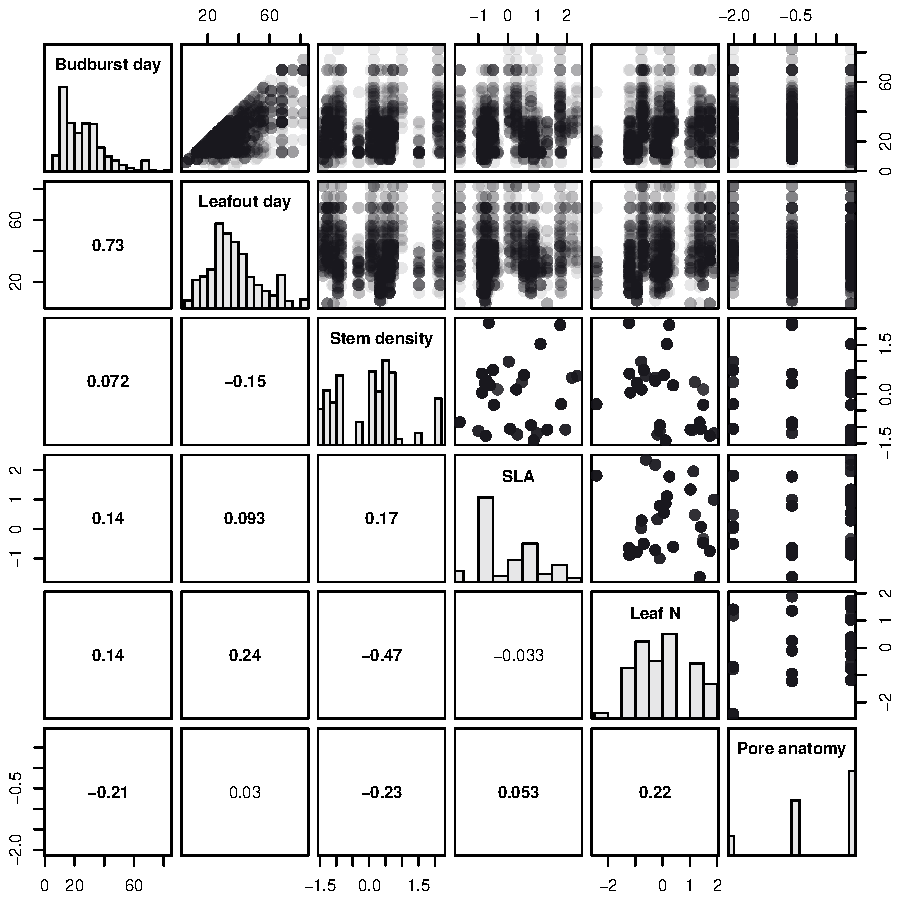
\includegraphics[scale=0.75]{traitpairs}
\end{figure}

\begin{figure}
\caption{Model estimates of budburst, including species-level effects.}
\label{figS2}
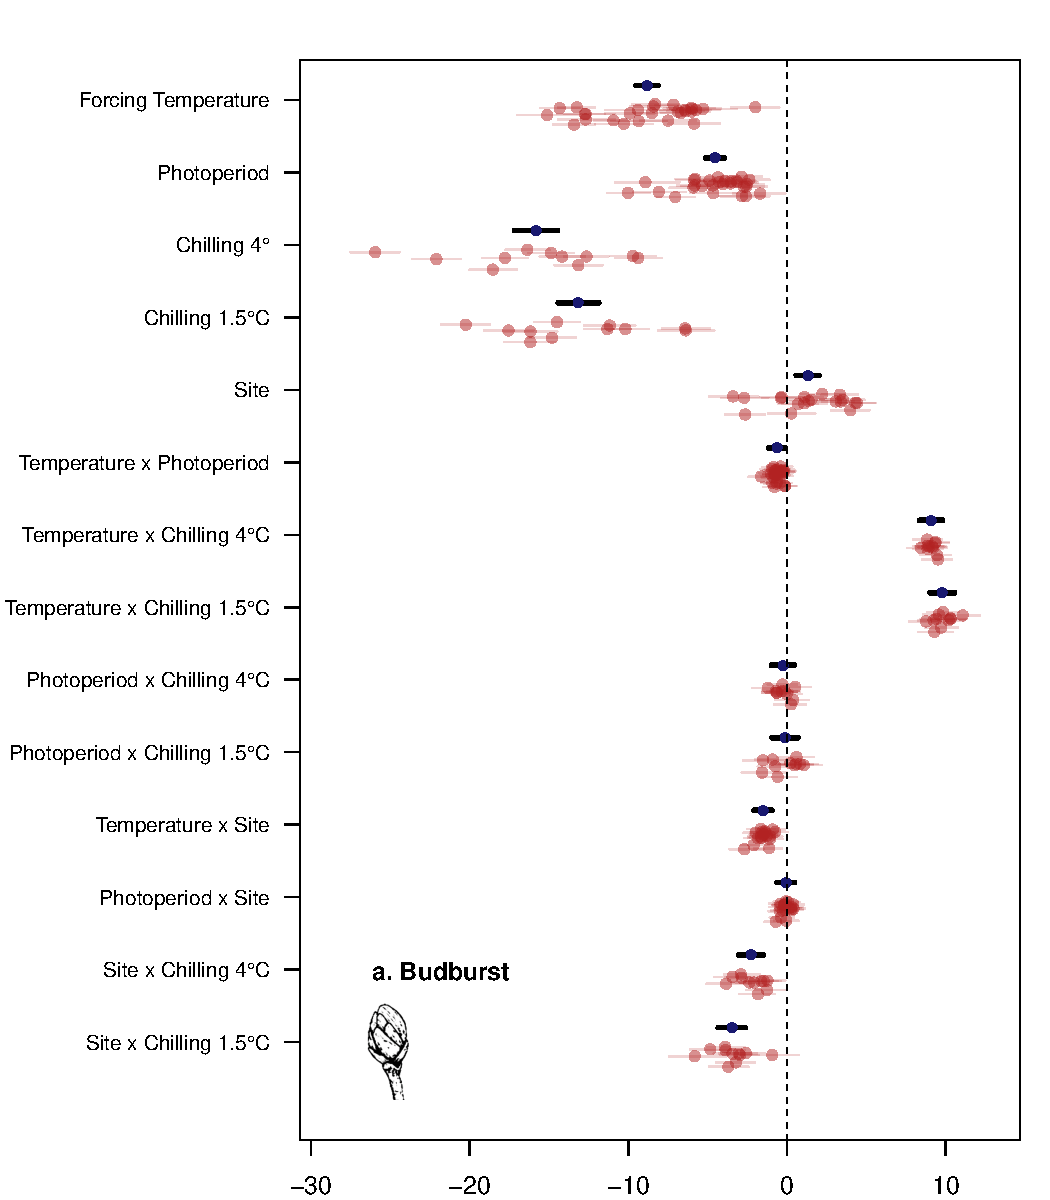
\includegraphics[scale=0.75, page=1]{Fig1_bb_lo+sp}
\end{figure}

\clearpage

\begin{figure}
\caption{Model estimates of leafout, including species-level effects.}
\label{figS3}
\includegraphics[scale=0.75, page=2]{Fig1_bb_lo+sp}
\end{figure}

\begin{figure}
\caption{Model estimates of sensitivity to warming, photoperiod, and chilling, compared to day of budburst (upper panels) or leafout (lower panels) across all experimental conditions.}
\label{figS4}
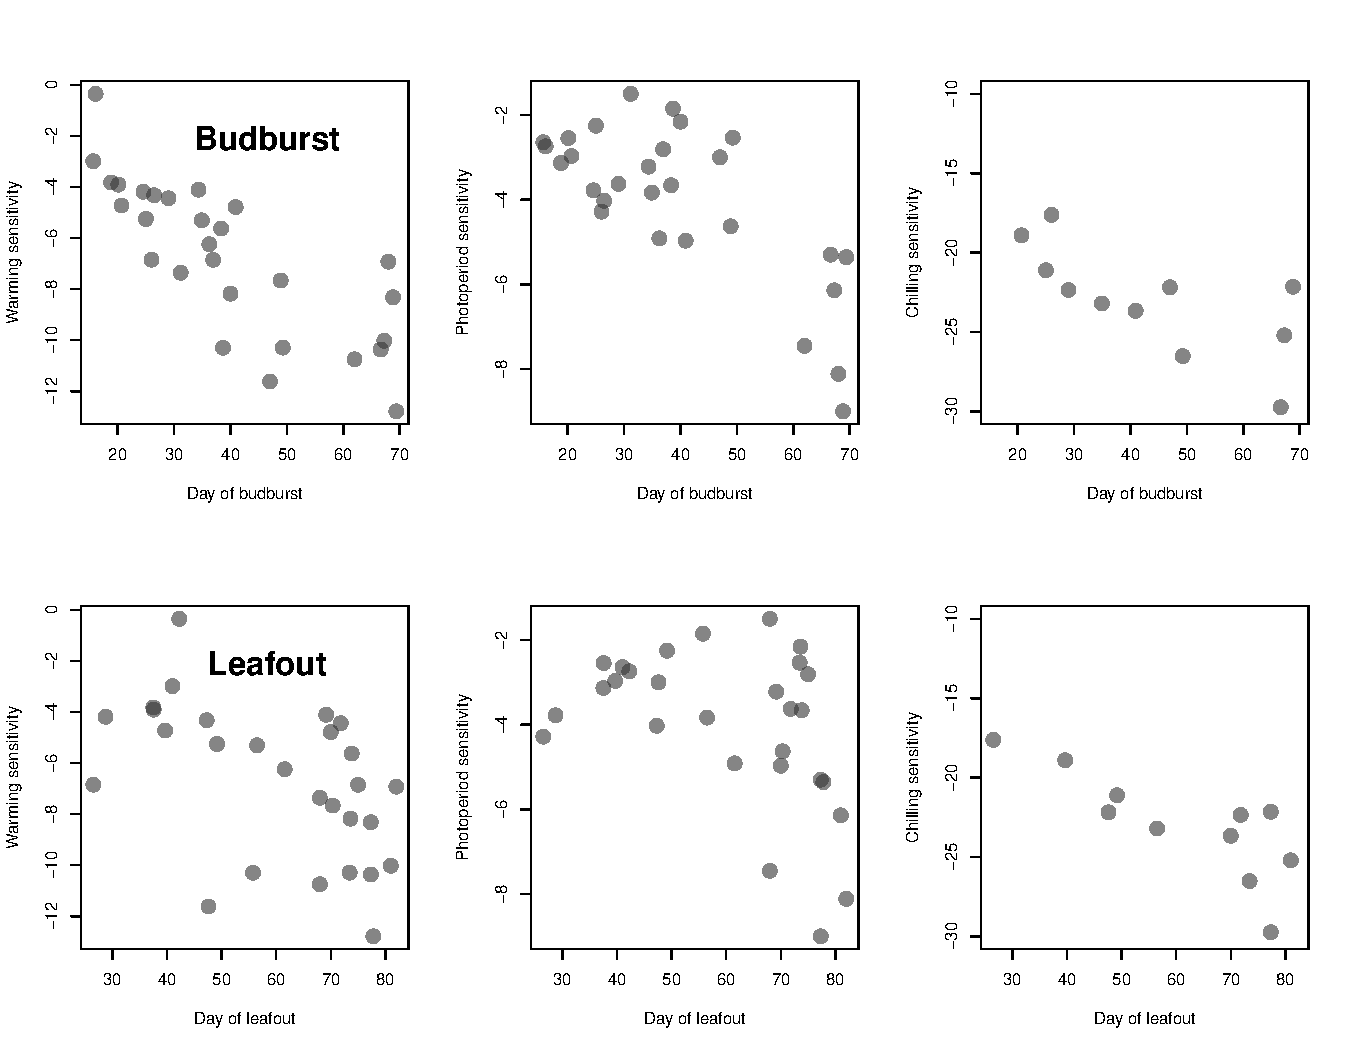
\includegraphics[scale=0.75]{Sens_vs_day}
\end{figure}

\end{document}
